\section{Real Scalar Field Theory III, Dirac Field Theory}
Last time, we discussed a real scalar field theory, and demonstrated some consequences of translational and Lorentz symmetry (Poincare symmetries). The discussion was a bit abstract; let's now move to a more concrete calculation; we claimed things were analytic last class, but let's actually show this via an example.

\subsection{Deriving the Free-Field Feynman Propagator}
Recall the solutions:
\begin{equation}
    \varphi(x) = \int \frac{d^3k}{\sqrt{(2\pi)^32\omega(\v{k})}} \left(e^{i\v{k} \cdot \v{x} - i\omega(\v{k})x^0}a(\v{k}) + e^{-i\v{k}\cdot\v{x} + i\omega(\v{k})t}a^\dag(\v{k})\right)
\end{equation}
these were solutions to the field equation, and is a solution to the QFT if we enforce the equal-time commutation relations on $a, a^\dag$.

Having an exact solution for free fields, we can look at some simple correlation functions and see what they look like. It shouldn't be difficult to convince yourself that after finding the two-point correlation functions for free fields, you can find arbitrary $N$-point correlation functions. Let us begin there; it is important enough to get its own name; the \emph{Feynman propagator}. We denote it as:
\begin{equation}
    \Delta(x, y) = \left.\bra{0}J\varphi(x)\varphi(y)\ket{0} \right|_{\lambda=0}
\end{equation}
The two point function of the interacting theory is also interesting (and has its own name), and we will get to this soon. We can write the Feynman propagator as follows:
\begin{equation}
    \Delta(x, y) = \theta(x^0 - y^0)\bra{0}\varphi(x)\varphi(y)\ket{0} + \theta(y^0 - x^0)\bra{0}\varphi(y)\varphi(x)\ket{0}
\end{equation}
where the Heaviside step functions enforce the time ordering. We can take and plug in our expressions for $\varphi$ and plug them in; using the creation/annhilation relations, this is sufficient to do this calculation. Doing so, we find:
\begin{equation}
    \Delta(x, y) = \theta(x^0 - y^0) \int \frac{d^3k}{(2\pi)^3 2\omega(\v{k})}e^{i\v{k} \cdot (\v{x} - \v{y}) - i\omega(x^0 - y^0)} + \theta(y^0 - x^0)\int \frac{d^3k}{(2\pi)^3 2\omega(\v{k})}e^{-i\v{k} \cdot (\v{x} - \v{y}) + i\omega(x^0 - y^0)}
\end{equation}
notice how the second term is just the first term with $x, y$ interchanged; the time ordering makes things symmetric as a function of the coordinates. Last time, we discussed the analyticity of Wightman functions; the first term is analytic in the lower half plane, and then has support in the the right half plane due to the Heaviside, so is analytic in the fourth quadrant. The second term is analytic in the upper half plane and has support in the left half plane due to the Heaviside, so is analytic in the second quadrant. This turns out to be a very useful observation; this is because this allows us to change what we mean by time by adding a complex number to it (analytically continuing where the time goes); in some sense putting $t \mapsto it$. This is known as a Wick rotation, and doing this we can make Minkowski space look like Euclidean space. This can be a useful starting point for our field theory; it is technically a wonderful thing! We get to work with a much nicer metric without the minus sign.

\begin{figure}[htbp]
    \centering
    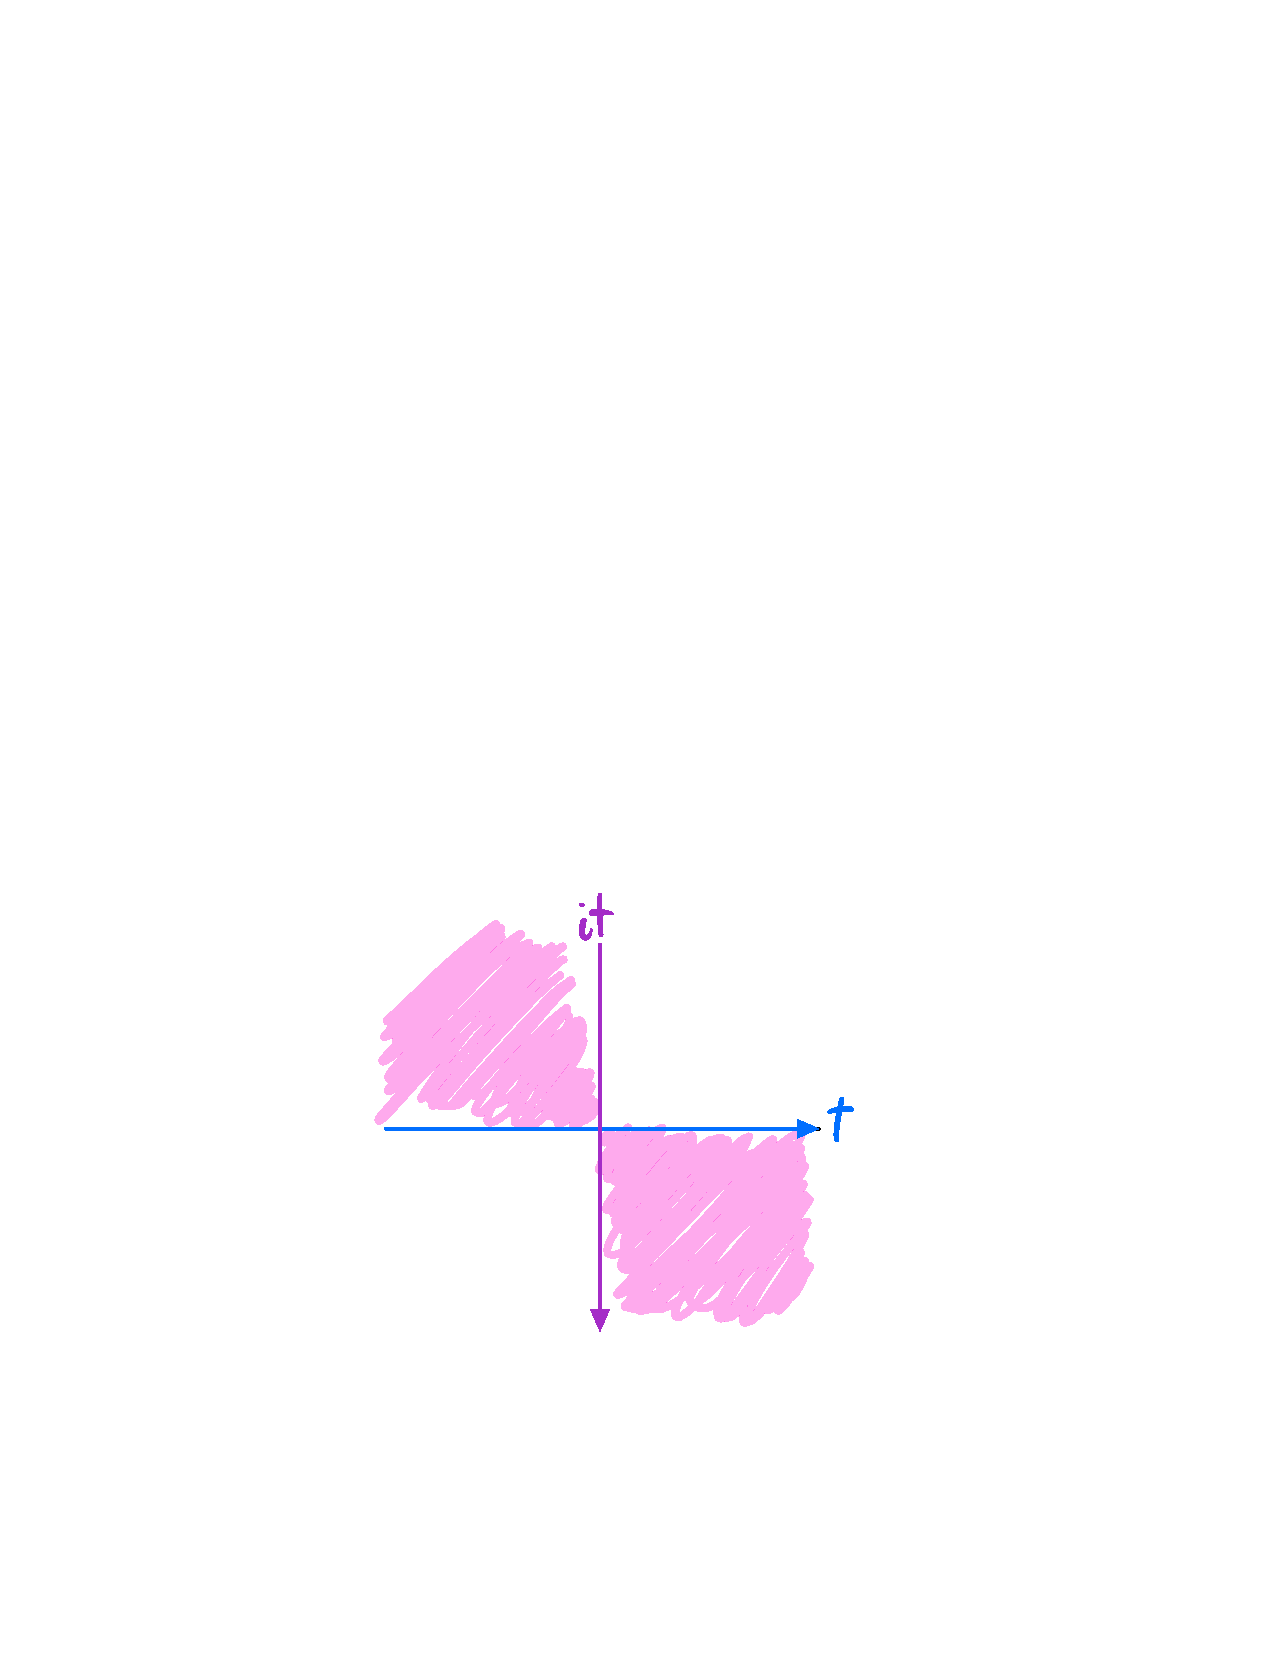
\includegraphics[scale=0.8]{Images/fig-analyticregionwickrotation.pdf}
    \caption{The first term in the above integral is analytic in the fourth quadrant and the second term in the above integral is analytic in the second quadrant. We can then take our contour integral for time which goes along the real axis, and rotate it so it lies on the imaginary axis (Wick rotation). Doing so, our Minkowski space looks Euclidean!}
    \label{fig-analyticregionwickrotation}
\end{figure}



\subsection{Another way to derive the Free-Field Feynman Propagator}
We have derived the two-point function, but not as it appears in most textbooks, or the most useful form for us. We could do it the technical/long way or we can take a pedagogical shortcut. Recall the solution to our QFT solves the field equation:
\begin{equation}
    (-\p^2 + m^2)\varphi(x) = 0
\end{equation}
So what happens if we take this operator and operate it on the time-ordered two-point function? We would find:
\begin{equation}
    (-\p^2 + m^2)\bra{0}J\varphi(x)\varphi(y)\ket{0} = 0.
\end{equation}
Can we just pull this in and get zero? No, not quite; $\p^2$ contains time derivatives, and we have a time ordering of the fields inside the expectation value; we need to take this into account. Let's consider the time derivative:
\begin{equation}
    \dpd{^2}{(x^0)^2}\bra{0}J\varphi(x)\varphi(y)\ket{0}
\end{equation}
and pulling this in and using the product rule and that the derivative of a step function is the dirac delta, as well as the equal time commutation relations:
\begin{equation}
    \begin{split}
        \dpd{^2}{(x^0)^2}\bra{0}J\varphi(x)\varphi(y)\ket{0} &= \dpd{}{x^0}\left(\bra{0}J\dpd{}{x^0}\varphi(x)\varphi(y)\ket{0} + \cancel{\delta(x^0 - y^0)\bra{0}[\varphi(x), \varphi(y)]\ket{0}}\right)
        \\ &= \bra{0}J\dpd{^2\varphi(x)}{(x^0)^2}\varphi(y)\ket{0} + \delta(x^0 - y^0)\bra{0}[\dpd{}{x^0}\varphi(x), \varphi(y)]\ket{0} = -i\delta(x - y)
    \end{split}
\end{equation}
We therefore learn:
\begin{equation}
    (-\p^2 + m^2)\Delta(x, y) = -i\delta(x - y)
\end{equation}
so $\Delta(x, y)$ is a Green's function! Note that this would not be the case for interacting fields as the wave equation is modified. So, we can short circuit all of our work that we have been doing as we can just find a solution to the Green's function equation above. Naively, we can solve this using a Fourier transform so we find:
\begin{equation}
    \Delta(x, y) = \int \frac{d^4k}{(2\pi)^4}e^{ik_\mu(x - y)^\mu} - \frac{i}{k^2 + m^2} 
\end{equation}
where $k^2 = \v{k}^2 - (k^0)^2$. Here the problem becomes apparent; we have a singularity in the above expression. We need to enforce boundary conditions. We take the singularity at $k^0$ and resolve it by adding a small imaginary part into the denominator, in such a way such that when we do the $k^0$ integral (which we could do via Cauchy's integral theorem, if we like):
\begin{equation}
    \Delta(x, y) = \int \frac{d^4k}{(2\pi)^4}e^{ik_\mu(x - y)^\mu} - \frac{i}{k^2 + m^2 - i\e} 
\end{equation}
which fixes the ambiguity and gives us a time-ordered boundary condition. We leave it as an exercise (though it is detailed in the textbook) for how we can write this as something that has two poles, then use partial fractions to separate the two pole terms, and use Cauchy's integral formula to get to:
\begin{equation}
    \Delta(x, y) = \theta(x^0 - y^0) \int \frac{d^3k}{(2\pi)^3 2\omega(\v{k})}e^{i\v{k} \cdot (\v{x} - \v{y}) - i\omega(x^0 - y^0)} + \theta(y^0 - x^0)\int \frac{d^3k}{(2\pi)^3 2\omega(\v{k})}e^{-i\v{k} \cdot (\v{x} - \v{y}) + i\omega(x^0 - y^0)}
\end{equation}
The discussion of analyticity follows exactly as we had before as we have the same expression. There is also a comment we can make about $k^0$. We have poles on the real axis originally, which we add a small $+i\e$ to the denominator to shift them above/below it so we can integrate over the real axis. This enforces boundary conditions. 

We can also consider doing an path integral whose interior does not contain either of the poles (pictured below). Adding it to the integral along the real axis, and taking the boundary to infinity, we get an integral just along the imaginary axis; something that looks Euclidean. This turns out to be extremely useful when we do calculations; we go from a slightly fishy Minkowski space integral to a Euclidean integral that is completely well-defined.

\begin{figure}[htbp]
    \centering
    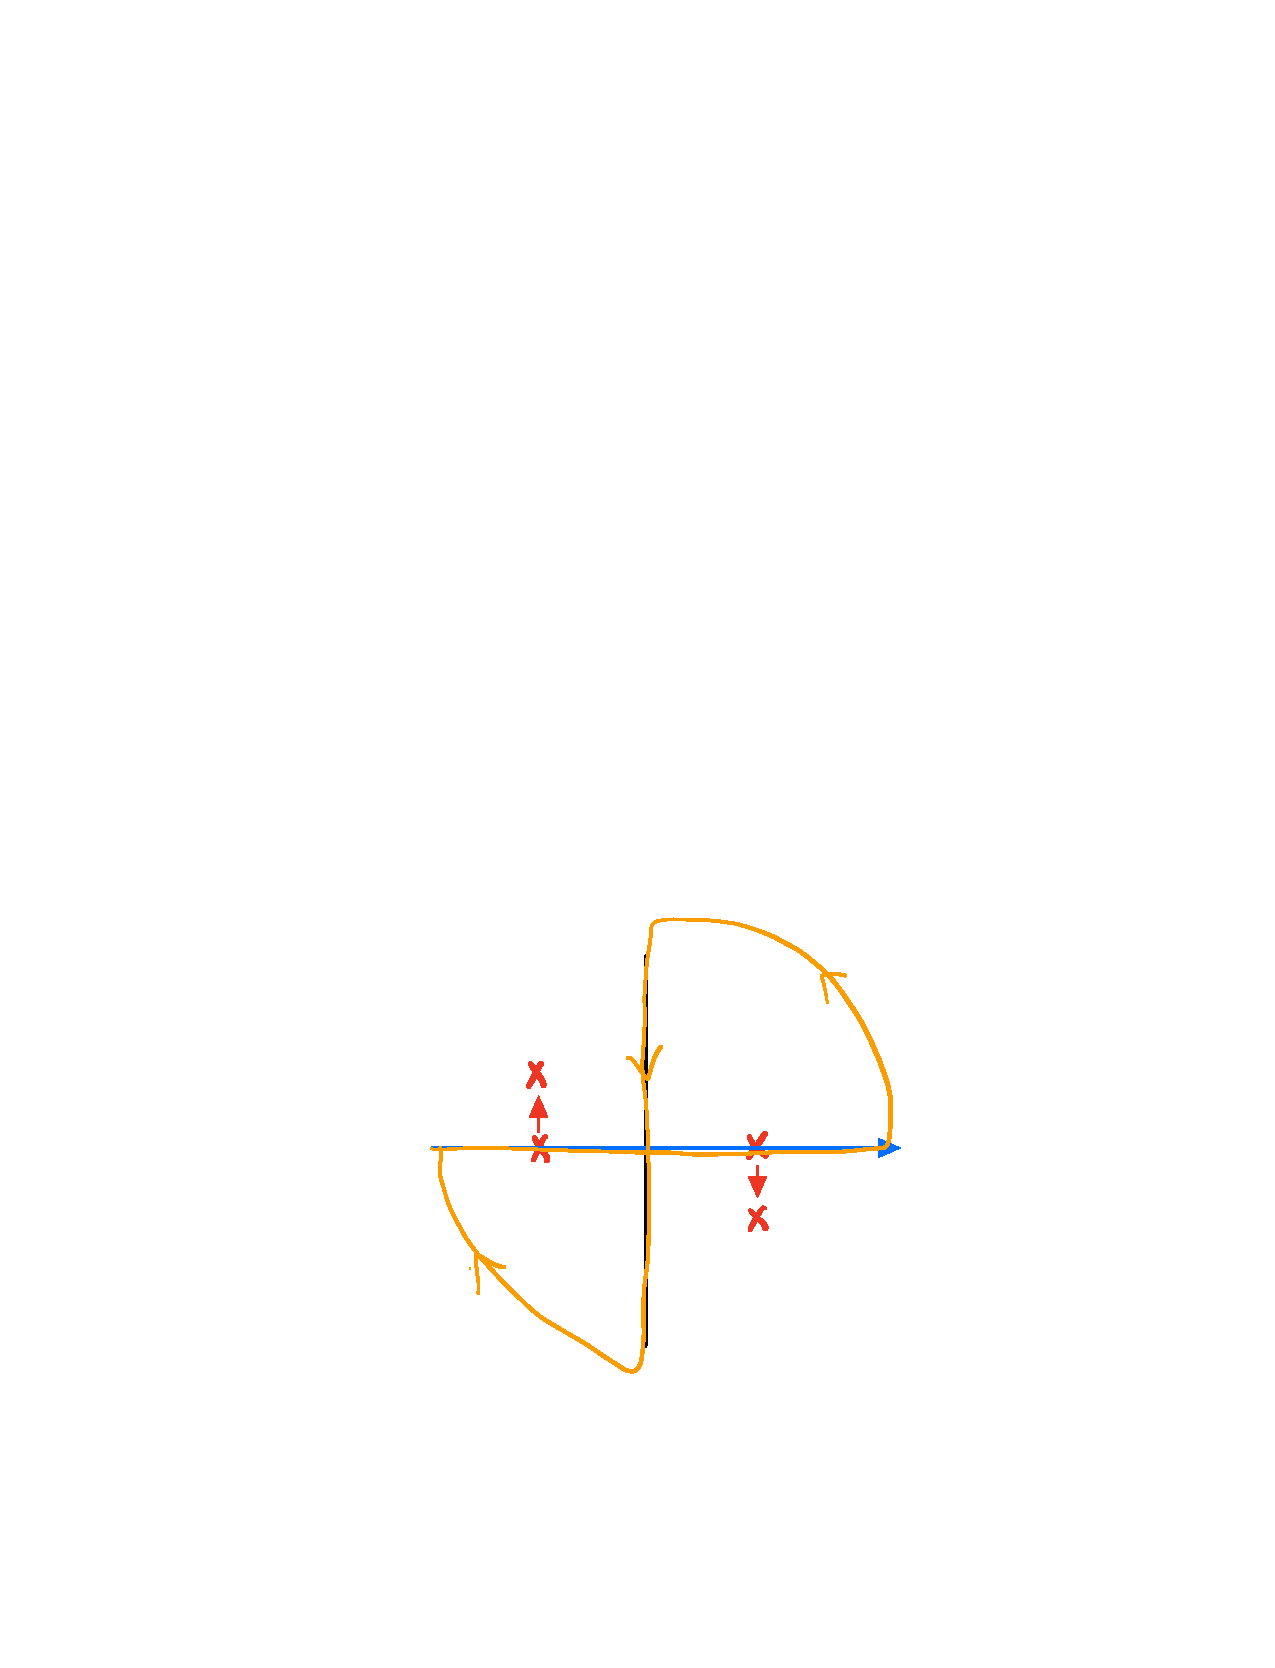
\includegraphics[scale=0.8]{Images/fig-propogatorcontour.pdf}
    \caption{The poles (in red) which originally sat on the time axis have been shifted above/below the real axis via the inclusion of the $-i\e$ in the denominatr of the propogator integral. This allows for a meaningful integral to be taken over the real axis. We can also consider a path integral whose interior contains none of the poles; adding this with the integral over the real axis, we obtain our integral over the imaginary time axis, wherein Minkowski space looks Euclidean.}
    \label{fig-propogatorcontour}
\end{figure}

A few other comments; recall in our discussion of wavepacket dispersion where we added two terms, one for particle and one for antiparticle. This is not the same as the addition of two terms we see here. We were seeing a different kind of Green's function, i.e. a retarded Green's functions (vs. the time-ordered Green's function we see here). This is the appropriate Green's function if we want the past to influence the future. This is a bit of an interesting subtle point; to get causality, we need to do a bit more work compared to what we have done here.

We can use some combinatorics to obtain all other correlation functions; so the free field scalar field theory is completely solved! We will put off studying the interacting field theory until we have a couple more free field theories under our belt. After this in the textbook, we have a chapter about emergent relativistic field theory. It will not be covered in lecture, but it is useful in studying relativistic field theories that go beyond particle physics (e.g. phonons, electrons in graphene). Field theories would be confined to a quite narrow range if we only look at the standard model; the condensed matter side of things offers some interesting cases of study! If we get to the end of the course and have discussed everything else, perhaps we can come back to it.

\subsection{Introduction to the Dirac Field}
There is a basic scalar field amidst the elementary particles - the celebrated Higgs field. The next step up adds spin to the mix (the scalar field has no spin); in particular spin-1/2 as the simplest one. This is the \emph{Dirac Field}, which describes fermions. Since it describes spin, we need another index which at least runs over two. But beyond this, we also need our causality arguments, which requires the existence of an antiparticle. The scalar field did not appear to have this; it did have a negative frequency branch, but this was not a different kind of particle, really. This could happen for dirac-looking field theories as well (though in this case this is not a dirac field, but instead we have majorana particles! which are their own antiparticles). A direct example; electrons and electron holes in the Fermi sea.

The above discussion suggests that we need a 4-component wavefunction (2 spin states for the particle and antiparticle each). This would suggest the guess:
\begin{equation}
    H =? \m{\sqrt{p^2 + m^2} & 0 & 0 & 0 \\ 0 & \sqrt{p^2 + m^2} & 0 & 0 \\ 0 & 0 & -\sqrt{p^2 + m^2} & 0 \\ 0 & 0 & 0 & -\sqrt{p^2 + m^2}}
\end{equation}
but this is ugly, and the spin is basically trivial here; and we don't have a way of knowing that the spin is trivial unless we know things about group theory and representations of the Lorentz group. We would expect that there would be not just two degenerate spin states, as we have here (think relativistic corrections to the hydrogen spectrum!) So the above formula is not correct. Dirac came up with a better idea; can we find some matrices with the correct Hermiticity properties such that the eigenvalues are the same as what we have written above, and it is linear in momentum?
\begin{equation}
    H = i\gv{\alpha}\cdot \nabla + \beta m
\end{equation}
In writing this, Dirac discovered antiparticles; he was however extremely confused with this discovery (even after the experimental discovery of the proton...) It was confusing as it was brilliant. These matrices, in order to have the same spectra, have to be realized as a quaternion factorization of the original guess we had above. They obey the algebra:
\begin{equation}
    \set{\alpha^a, \alpha^b} = 2\delta^{ab}\mathbb{I}, \quad \beta^2 = \mathbb{I}, \quad \set{\alpha^a, \beta} = 0.
\end{equation}
and are Hermitian:
\begin{equation}
    (\alpha^a)^\dag = \alpha^a, \beta^\dag = \beta.
\end{equation}
These are the Dirac Matrices. To study time evolution, we take this Hamiltonian and put it into the Schrodinger equation:
\begin{equation}
    i\dpd{}{t}\psi = (i\gv{\alpha} \cdot \nabla + \beta m)\psi
\end{equation}
where all we have really done is substituted in the Schrodinger operator for the Dirac operator. If we were to derive this theory from the Lagrangian density, we would have something that looks very similar to the original Lagrangian density for our non-relativistic QFT:
\begin{equation}
    \L = i\psi^{\dag}_\sigma \dpd{}{t}\psi_\sigma + \ldots
\end{equation}
with the equal-time anticommutation relations:
\begin{equation}
    \{\psi_a(x), \psi^{\dag}_b(y)\}\delta(x^0 - y^0) = \delta(x - y)
\end{equation}
\begin{equation}
    \{\psi^\dag_a(x), \psi^{\dag}_b(y)\}\delta(x^0 - y^0) = \{\psi_a(x), \psi_b(y)\}\delta(x^0 - y^0) = 0.
\end{equation}

At this point, there is no reason to expect that the states are fermions; one way to figure this out would be that if we had bosons, we would have an unstable theory as we would fill up the negative energy states as much as we want. We need the Pauli principle to stabilize the Fermi sea and ensure that the negative energy states are already filled. Another more formal way to see this; if we use the commutation relations, we would find that the Hamiltonian is not bounded from below. Note that the Poisson bracket actually becomes modified in the case where we have anti-commuting vs. commuting classical fields.

Next time we explore solutions to this theory. Before then; a question; is this theory actually relativistic? We set up the equation such that the spectrum is relativistic with $\sqrt{p^2 + m^2}$. The details we have yet to work out, the answer will (of course) be yes, however.